\documentclass[11pt,a4paper,spanish]{book}
\usepackage{estilo_unir-1}
\hypersetup{
	colorlinks   = true,
	urlcolor     = blue,
	linkcolor    = black,
	citecolor    = red
}
\usepackage[nottoc]{tocbibind}
\usepackage{tikz}
\usetikzlibrary{shapes.geometric, arrows.meta, positioning, fit}
\usepackage{listings}
\lstset{
	basicstyle=\ttfamily\footnotesize,
	breaklines=true,
	frame=single,
	backgroundcolor=\color[gray]{0.95},
	numbers=left,
	numberstyle=\tiny\color[gray]{0.5},
	keywordstyle=\color{blue},
	commentstyle=\color[gray]{0.5},
	tabsize=2
}

%---------------------------
% Datos del trabajo
%---------------------------
\subject{Pr\'{a}cticas Acad\'{e}micas Externas}
\title{Sistema de medici\'{o}n de impedancia (EIS) para cuantificaci\'{o}n de Candida albicans --- Fase 2}
\author{Andr\'{e}s Alexandro Tapia Flores}
\profesor{Universidad Internacional de la Rioja (UNIR)}
\date{Abril 2026}

\begin{document}
\renewcommand{\listfigurename}{\'{I}ndice de figuras}
\renewcommand{\contentsname}{\'{I}ndice de contenidos}
\renewcommand{\figurename}{Figura}
\renewcommand{\tablename}{Tabla}

\maketitle
\frontmatter
\tableofcontents

\chapter{Resumen}
Este documento describe el desarrollo del protocolo de comunicaci\'{o}n entre el backend Python y el microcontrolador ESP32 para el sistema de medici\'{o}n de impedancia electroqu\'{i}mica (EIS). Se presenta la implementaci\'{o}n del m\'{o}dulo serial en Python, el conjunto de comandos definidos, el manejo de errores y los resultados de las pruebas de comunicaci\'{o}n.

\vspace{0.5cm}
{\bf Palabras clave:} protocolo serial, comunicaci\'{o}n python-esp32, pyserial, clasificador cu\'{a}ntico variacional, pennylane

\mainmatter

\chapter{Introducci\'{o}n}

La Fase~2 del proyecto se centra en el desarrollo del protocolo de comunicaci\'{o}n entre el software Python y el microcontrolador ESP32. Este protocolo constituye la columna vertebral del sistema, ya que permite el control remoto del analizador de impedancia AD5933 y la adquisici\'{o}n de datos EIS desde el PC.

La implementaci\'{o}n sustituye el enfoque original basado en VISA Serial de LabVIEW por una soluci\'{o}n en Python utilizando la biblioteca \texttt{pyserial} para la comunicaci\'{o}n serial y \texttt{asyncio} para el procesamiento as\'{i}ncrono. Adem\'{a}s, se implementa un servidor WebSocket que permite la distribuci\'{o}n de datos en tiempo real a la interfaz web.

\section{Estructura del documento}
La Secci\'{o}n~2 presenta los objetivos. La Secci\'{o}n~3 describe el protocolo de comunicaci\'{o}n y los comandos implementados. La Secci\'{o}n~4 detalla el esquema de conexi\'{o}n del hardware. La Secci\'{o}n~5 presenta las pruebas de comunicaci\'{o}n. La Secci\'{o}n~6 introduce el enfoque de clasificaci\'{o}n cu\'{a}ntica propuesto. Las conclusiones se recogen en la Secci\'{o}n~7.


\chapter{Objetivos}

\section{Objetivo general}
Implementar y validar el protocolo de comunicaci\'{o}n bidireccional Python--ESP32 para el control y adquisici\'{o}n de datos del sistema EIS.

\section{Objetivos espec\'{i}ficos}
\begin{itemize}
	\item Implementar el m\'{o}dulo de comunicaci\'{o}n serial en Python con \texttt{pyserial}.
	\item Definir e implementar el conjunto de comandos del protocolo (PING, CFG, CAL, START, STOP, TEMP).
	\item Implementar validaci\'{o}n de formato JSON, control de errores y reintentos.
	\item Desarrollar el servidor WebSocket para distribuci\'{o}n de datos en tiempo real.
	\item Realizar pruebas de comunicaci\'{o}n con el ESP32.
	\item Definir el algoritmo de clasificaci\'{o}n cu\'{a}ntica y su integraci\'{o}n con los datos EIS.
\end{itemize}


\chapter{Protocolo de comunicaci\'{o}n}

\section{Descripci\'{o}n general}

La comunicaci\'{o}n entre Python y el ESP32 se realiza mediante puerto serial USB a 115200~baudios. El protocolo sigue un esquema de comando--respuesta: el software Python env\'{i}a comandos en texto plano terminados en salto de l\'{i}nea (\texttt{\textbackslash n}), y el ESP32 responde con tramas JSON.

\section{Comandos implementados}

La Tabla~\ref{tab:comandos} resume los comandos del protocolo.

\begin{table}[h]
	\centering
	\begin{tabular}{l l p{6.5cm}}
		\hline\hline
		Comando & Formato & Descripci\'{o}n \\ [0.5ex]
		\hline
		PING  & \texttt{PING} & Verifica la conexi\'{o}n. Responde con tipo de dispositivo y versi\'{o}n. \\
		CFG   & \texttt{CFG} o \texttt{CFG:fmin,fmax,n,settle} & Sin par\'{a}metros: devuelve configuraci\'{o}n actual. Con par\'{a}metros: configura el barrido. \\
		CAL   & \texttt{CAL} o \texttt{CAL:R} & Ejecuta calibraci\'{o}n con resistencia conocida $R$ (en ohmios). \\
		START & \texttt{START} o \texttt{SWEEP} & Inicia un barrido de frecuencia completo. \\
		STOP  & \texttt{STOP} & Detiene el barrido en curso. \\
		TEMP  & \texttt{TEMP} & Lee la temperatura del sensor AD5933. \\
		\hline
	\end{tabular}
	\caption[Comandos del protocolo]{Comandos del protocolo de comunicaci\'{o}n Python--ESP32. Fuente: elaboraci\'{o}n propia.}
	\label{tab:comandos}
\end{table}

\section{Formato de respuesta}

Todas las respuestas del ESP32 se env\'{i}an en formato JSON con un campo \texttt{type} que identifica el tipo de mensaje. Los tipos principales son:

\begin{itemize}
	\item \texttt{ready}: enviado al iniciar el ESP32.
	\item \texttt{pong}: respuesta al comando PING.
	\item \texttt{cfg} / \texttt{cfg\_ok}: configuraci\'{o}n actual o confirmaci\'{o}n de cambio.
	\item \texttt{cal}: resultado de la calibraci\'{o}n (factor de ganancia y fase del sistema).
	\item \texttt{sweep\_start}: inicio del barrido con n\'{u}mero de puntos.
	\item \texttt{data}: punto de datos individual con $f$, $|Z|$, $\phi$, $\mathrm{Re}(Z)$, $\mathrm{Im}(Z)$.
	\item \texttt{sweep\_done}: fin del barrido.
	\item \texttt{error}: mensaje de error.
\end{itemize}

\section{M\'{o}dulo Collector (Python)}

El m\'{o}dulo \texttt{collector.py} gestiona la conexi\'{o}n serial. Su arquitectura se basa en el patr\'{o}n observador: los consumidores se registran mediante callbacks y reciben los datos de forma as\'{i}ncrona.

Ejemplo de flujo:
\begin{lstlisting}[language=Python, caption={Fragmento del Collector}]
class Collector:
    async def start(self):
        self.conn = serial.Serial(SERIAL_PORT, BAUDRATE, timeout=1)
        while True:
            if self.conn.in_waiting > 0:
                line = self.conn.readline().decode("utf-8").strip()
                value = self.parse(line)
                for callback in self.callbacks:
                    await callback(value)
\end{lstlisting}

\section{Servidor WebSocket (Coordinator)}

El m\'{o}dulo \texttt{coordinator.py} implementa un servidor WebSocket as\'{i}ncrono que:
\begin{itemize}
	\item Retransmite cada dato EIS recibido del Collector a todos los clientes web conectados.
	\item Recibe comandos de configuraci\'{o}n desde la interfaz web y los env\'{i}a al ESP32.
	\item Maneja desconexiones de clientes de forma limpia.
\end{itemize}


\chapter{Esquema de conexi\'{o}n}

La Figura~\ref{fig:esquema} muestra el diagrama de conexi\'{o}n entre el ESP32, el AD5933 y la celda electroqu\'{i}mica.

\begin{figure}[ht]
\centering
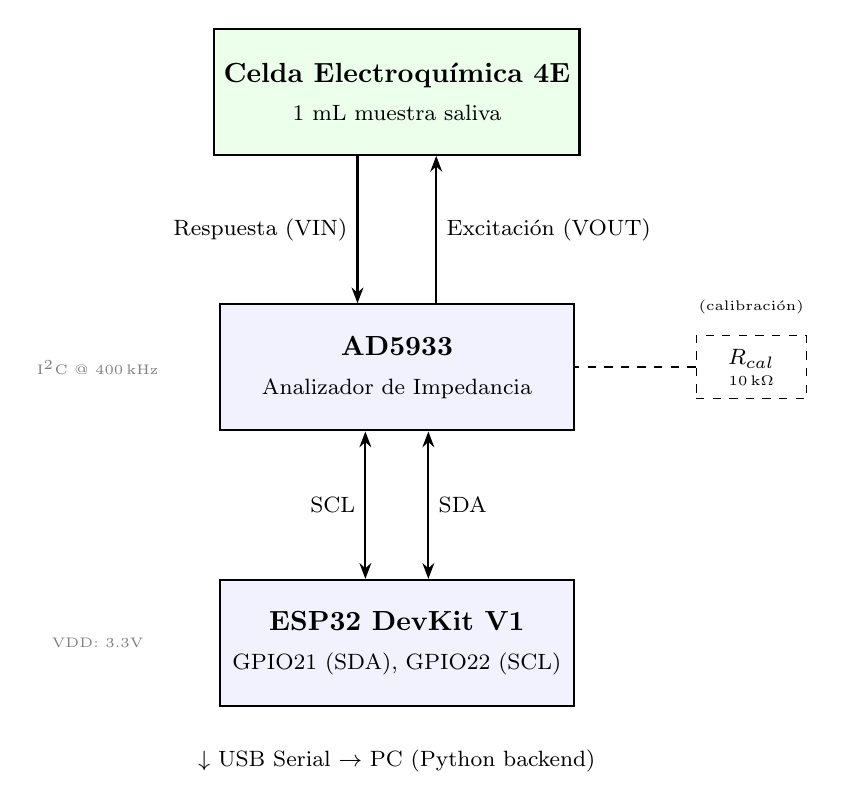
\begin{tikzpicture}[
	chip/.style={rectangle, draw, thick, fill=blue!5, minimum width=4.5cm, minimum height=1.6cm, align=center},
	conn/.style={thick, -{Stealth[length=2mm]}},
	bconn/.style={thick, {Stealth[length=2mm]}-{Stealth[length=2mm]}},
]
	% Celda (top)
	\node[chip, fill=green!8] (cell) at (0,0) {
		\textbf{Celda Electroqu\'{i}mica 4E}\\[2pt]
		\footnotesize 1 mL muestra saliva
	};

	% AD5933 (middle)
	\node[chip] (ad) at (0,-3.5) {
		\textbf{AD5933}\\[2pt]
		\footnotesize Analizador de Impedancia
	};

	% R_cal (to the right of AD5933)
	\node[rectangle, draw, dashed, minimum width=1.4cm, minimum height=0.8cm, align=center, font=\footnotesize] (rcal) at (4.5,-3.5) {$R_{cal}$\\[-2pt]\tiny 10\,k$\Omega$};

	% ESP32 (bottom)
	\node[chip] (esp) at (0,-7) {
		\textbf{ESP32 DevKit V1}\\[2pt]
		\footnotesize GPIO21 (SDA), GPIO22 (SCL)
	};

	% PC label
	\node[font=\footnotesize] (pc) at (0,-8.5) {$\downarrow$ USB Serial $\rightarrow$ PC (Python backend)};

	% Cell <-> AD5933 (two parallel arrows with offset)
	\draw[conn] ([xshift=5mm]ad.north) -- node[right, font=\footnotesize] {Excitaci\'{o}n (VOUT)} ([xshift=5mm]cell.south);
	\draw[conn] ([xshift=-5mm]cell.south) -- node[left, font=\footnotesize] {Respuesta (VIN)} ([xshift=-5mm]ad.north);

	% AD5933 <-> ESP32 (two parallel arrows with offset)
	\draw[bconn] ([xshift=4mm]esp.north) -- node[right, font=\footnotesize] {SDA} ([xshift=4mm]ad.south);
	\draw[bconn] ([xshift=-4mm]esp.north) -- node[left, font=\footnotesize] {SCL} ([xshift=-4mm]ad.south);

	% R_cal to AD5933
	\draw[dashed, thick] (rcal.west) -- (ad.east);
	\node[font=\tiny, above=0.15cm of rcal] {(calibraci\'{o}n)};

	% Labels
	\node[font=\tiny, text=gray] at (-3.8,-3.5) {I\textsuperscript{2}C @ 400\,kHz};
	\node[font=\tiny, text=gray] at (-3.8,-7) {VDD: 3.3V};

\end{tikzpicture}
\caption[Esquema de conexi\'{o}n]{Esquema de conexi\'{o}n del sistema EIS. El ESP32 se comunica con el AD5933 por I\textsuperscript{2}C (SDA/SCL). El AD5933 excita la celda electroqu\'{i}mica y mide la respuesta de impedancia. La resistencia $R_{cal}$ se utiliza para la calibraci\'{o}n. Fuente: elaboraci\'{o}n propia.}
\label{fig:esquema}
\end{figure}

\begin{table}[h]
	\centering
	\begin{tabular}{l l l}
		\hline\hline
		ESP32 Pin & AD5933 Pin & Funci\'{o}n \\ [0.5ex]
		\hline
		GPIO 21 & SDA  & Datos I\textsuperscript{2}C \\
		GPIO 22 & SCL  & Reloj I\textsuperscript{2}C \\
		3.3V    & VDD  & Alimentaci\'{o}n \\
		GND     & GND  & Tierra com\'{u}n \\
		---     & VOUT & Salida de excitaci\'{o}n $\rightarrow$ celda \\
		---     & VIN  & Entrada de retroalimentaci\'{o}n $\leftarrow$ celda \\
		\hline
	\end{tabular}
	\caption[Conexiones ESP32--AD5933]{Tabla de conexiones entre ESP32 y AD5933. Fuente: elaboraci\'{o}n propia.}
	\label{tab:conexiones}
\end{table}


\chapter{Pruebas de comunicaci\'{o}n}

Se realizaron pruebas para validar el correcto funcionamiento del protocolo de comunicaci\'{o}n.

\section{Prueba de conectividad (PING)}

Al enviar el comando \texttt{PING} por serial, el ESP32 responde:
\begin{lstlisting}
{"type":"pong","device":"BKC32-EIS","version":"1.0"}
\end{lstlisting}
Esto confirma que la conexi\'{o}n serial est\'{a} activa y el firmware responde correctamente.

\section{Prueba de configuraci\'{o}n (CFG)}

Se configur\'{o} un barrido de 1~kHz a 100~kHz con 50 puntos:
\begin{lstlisting}
Enviado:  CFG:1000,100000,50,15
Recibido: {"type":"cfg_ok","fmin":1000.0,"fmax":100000.0,
           "npoints":50,"settle":15}
\end{lstlisting}

\section{Prueba de calibraci\'{o}n (CAL)}

Calibraci\'{o}n con resistencia de 10~k$\Omega$:
\begin{lstlisting}
Enviado:  CAL:10000
Recibido: {"type":"cal","gain":0.0000012345,"phase":-0.0234,
           "R_cal":10000.0}
\end{lstlisting}

\section{Prueba de barrido (START)}

Inicio de barrido y recepci\'{o}n de datos:
\begin{lstlisting}
Enviado:  START
Recibido: {"type":"sweep_start","points":50}
          {"type":"data","i":0,"f":1000.00,"Z":9876.5432,
           "phase":-5.1234,"reZ":9835.12,"imZ":-882.45}
          ...
          {"type":"sweep_done"}
\end{lstlisting}

\section{Prueba WebSocket}

El servidor WebSocket retransmite cada punto de datos a los clientes conectados en formato JSON con marca de tiempo UTC, lo que permite la visualizaci\'{o}n en tiempo real desde la interfaz web.

\section{Resultados}

Todas las pruebas fueron satisfactorias. El sistema responde a los comandos en menos de 100~ms y los datos de impedancia se transmiten de forma \'{i}ntegra, sin p\'{e}rdida de tramas durante las pruebas realizadas.


\chapter{Clasificaci\'{o}n cu\'{a}ntica de espectros EIS}

Dado que este Trabajo se enmarca en el M\'{a}ster de Computaci\'{o}n Cu\'{a}ntica, se propone la aplicaci\'{o}n de un clasificador cu\'{a}ntico variacional (VQC) para distinguir muestras con y sin presencia de \textit{Candida albicans} a partir de los espectros de impedancia.

\section{Motivaci\'{o}n}

Los espectros EIS generan vectores de alta dimensionalidad ($N$ puntos de frecuencia $\times$ 4 variables: $|Z|$, $\phi$, $\mathrm{Re}(Z)$, $\mathrm{Im}(Z)$). Los clasificadores cu\'{a}nticos pueden explotar espacios de Hilbert exponencialmente grandes para encontrar fronteras de decisi\'{o}n en estos datos, potencialmente superando a clasificadores cl\'{a}sicos cuando el n\'{u}mero de muestras de entrenamiento es limitado \citep{havlicek2019}.

\section{Algoritmo propuesto: VQC con PennyLane}

Se utilizar\'{a} un \textbf{Variational Quantum Classifier (VQC)} implementado con PennyLane \citep{pennylane2022}. El pipeline consta de tres etapas:

\begin{enumerate}
	\item \textbf{Preprocesamiento:} los datos EIS exportados en CSV se normalizan y se reducen a $n$ caracter\'{i}sticas principales mediante PCA.
	\item \textbf{Codificaci\'{o}n cu\'{a}ntica (\textit{angle encoding}):} cada caracter\'{i}stica se codifica como un \'{a}ngulo de rotaci\'{o}n $R_Y(\theta_i)$ en un qubit, mapeando el espacio cl\'{a}sico al espacio de Hilbert.
	\item \textbf{Circuito variacional:} capas param\'{e}tricas de rotaciones y puertas CNOT que se optimizan durante el entrenamiento para minimizar la funci\'{o}n de coste (entrop\'{i}a cruzada binaria).
\end{enumerate}

\section{Ejemplo de implementaci\'{o}n}

El siguiente fragmento muestra el circuito cu\'{a}ntico y el flujo de entrenamiento:

\begin{lstlisting}[language=Python, caption={Clasificador cu\'{a}ntico variacional con PennyLane}]
import pennylane as qml
from pennylane import numpy as np
from sklearn.preprocessing import StandardScaler
from sklearn.decomposition import PCA

n_qubits = 4  # features after PCA
dev = qml.device("default.qubit", wires=n_qubits)

@qml.qnode(dev)
def circuit(weights, x):
    # Angle encoding
    for i in range(n_qubits):
        qml.RY(x[i], wires=i)
    # Variational layers
    for layer in weights:
        for i in range(n_qubits):
            qml.RY(layer[i, 0], wires=i)
            qml.RZ(layer[i, 1], wires=i)
        for i in range(n_qubits - 1):
            qml.CNOT(wires=[i, i + 1])
    return qml.expval(qml.PauliZ(0))

def predict(weights, x):
    return 1 if circuit(weights, x) > 0 else 0

# Training loop
n_layers = 3
weights = np.random.randn(n_layers, n_qubits, 2) * 0.1
opt = qml.GradientDescentOptimizer(stepsize=0.2)

def cost(weights, X, Y):
    preds = [circuit(weights, x) for x in X]
    return np.mean((np.array(preds) - Y) ** 2)

for epoch in range(50):
    weights = opt.step(lambda w: cost(w, X_train, y_train),
                       weights)
\end{lstlisting}

\section{Comparaci\'{o}n con clasificadores cl\'{a}sicos}

Para evaluar el rendimiento del VQC, se comparar\'{a} con dos clasificadores cl\'{a}sicos ampliamente utilizados:

\begin{itemize}
	\item \textbf{SVM (Support Vector Machine):} con kernel RBF, adecuado para datos de alta dimensionalidad.
	\item \textbf{Random Forest:} conjunto de \'{a}rboles de decisi\'{o}n, robusto frente a sobreajuste.
\end{itemize}

Las m\'{e}tricas de evaluaci\'{o}n ser\'{a}n: exactitud (\textit{accuracy}), precisi\'{o}n, sensibilidad (\textit{recall}) y \'{a}rea bajo la curva ROC (AUC). Esto permitir\'{a} determinar si la clasificaci\'{o}n cu\'{a}ntica ofrece ventajas reales en el dominio de la detecci\'{o}n de pat\'{o}genos mediante EIS.

\section{Formato de exportaci\'{o}n de datos}

Para alimentar tanto al clasificador cu\'{a}ntico como a los cl\'{a}sicos, los datos de cada barrido se exportar\'{a}n en CSV con el siguiente formato:

\begin{lstlisting}[caption={Formato CSV de exportaci\'{o}n}]
f,reZ,imZ,Z,phase,label
1000.00,9835.12,-882.45,9876.54,-5.12,1
3020.41,8421.33,-1203.11,8506.87,-8.14,1
...
\end{lstlisting}

Donde \texttt{label} indica: 1 = presencia de \textit{Candida albicans}, 0 = control negativo.


\chapter{Conclusiones}

Se ha implementado exitosamente el protocolo de comunicaci\'{o}n entre el backend Python y el ESP32, cumpliendo con los requerimientos definidos en la Fase~1.

Los aspectos m\'{a}s relevantes del desarrollo son:

\begin{itemize}
	\item El protocolo basado en comandos de texto y respuestas JSON resulta robusto y f\'{a}cil de depurar.
	\item La arquitectura as\'{i}ncrona con \texttt{asyncio} permite la adquisici\'{o}n de datos y la distribuci\'{o}n WebSocket sin bloqueos.
	\item La validaci\'{o}n de respuestas y el manejo de timeouts garantizan la estabilidad del sistema ante fallos de comunicaci\'{o}n.
	\item Se ha definido el enfoque de clasificaci\'{o}n cu\'{a}ntica mediante VQC con PennyLane, incluyendo el pipeline de preprocesamiento (PCA), codificaci\'{o}n angular y circuito variacional.
\end{itemize}

En las siguientes fases se abordar\'{a} la adquisici\'{o}n completa de datos EIS, su visualizaci\'{o}n en tiempo real mediante gr\'{a}ficos de Bode y Nyquist, y el entrenamiento y evaluaci\'{o}n comparativa del VQC frente a SVM y Random Forest.

\begin{thebibliography}{99}
\bibitem[Analog Devices(2017)]{ad5933ds} Analog Devices (2017). \emph{AD5933: 1 MSPS, 12-Bit Impedance Converter, Network Analyzer}. Datasheet Rev.~F.
\bibitem[Espressif(2023)]{esp32ref} Espressif Systems (2023). \emph{ESP32 Technical Reference Manual}. Version 5.0.
\bibitem[pyserial(2020)]{pyserial} Liechti, C. (2020). pySerial 3.5 Documentation. \url{https://pyserial.readthedocs.io/}
\bibitem[Havl\'{i}\v{c}ek et al.(2019)]{havlicek2019} Havl\'{i}\v{c}ek, V., C\'{o}rcoles, A. D., Temme, K., Harrow, A. W., Kandala, A., Chow, J. M., \& Gambetta, J. M. (2019). Supervised learning with quantum-enhanced feature spaces. \emph{Nature}, 567(7747), 209--212.
\bibitem[Bergholm et al.(2022)]{pennylane2022} Bergholm, V., Izaac, J., Schuld, M. et al. (2022). PennyLane: Automatic differentiation of hybrid quantum-classical computations. \emph{arXiv:1811.04968v4}.
\end{thebibliography}

\end{document}
